\documentclass[conference]{IEEEtran}
\IEEEoverridecommandlockouts
\usepackage{graphicx}
\usepackage[colorlinks = true,
            linkcolor = black,
            urlcolor  = blue,
            citecolor = black,
            anchorcolor = blue]{hyperref}
\usepackage{amsmath,amssymb,amsfonts, mathtools}
\usepackage{algorithmic}
\usepackage{textcomp}
\usepackage{lipsum}                     
\usepackage{xargs}                      
\usepackage[pdftex,dvipsnames, table]{xcolor}  
\usepackage[table]{xcolor}
\usepackage{float}
\usepackage{subcaption}
\usepackage{stfloats}
\usepackage{bbm}
\usepackage[
backend=biber,
style=numeric,
sorting=ynt
]{biblatex}
\addbibresource[]{misc/references.bib}

\rowcolors{2}{gray!10}{white}

\newcommand{\titlecol}{\cellcolor{gray!30}}

% 
\usepackage[colorinlistoftodos,prependcaption,textsize=tiny]{todonotes}
\newcommandx{\unfinished}[2][1=]{\todo[linecolor=red,backgroundcolor=red!25,bordercolor=red,#1]{#2}}
\newcommandx{\change}[2][1=]{\todo[linecolor=blue,backgroundcolor=blue!25,bordercolor=blue,#1]{#2}}
\newcommandx{\info}[2][1=]{\todo[linecolor=OliveGreen,backgroundcolor=OliveGreen!25,bordercolor=OliveGreen,#1]{#2}}
\newcommandx{\improvement}[2][1=]{\todo[linecolor=Plum,backgroundcolor=Plum!25,bordercolor=Plum,#1]{#2}}
\newcommandx{\thiswillnotshow}[2][1=]{\todo[disable,#1]{#2}}

\begin{document}
\title{Security Analysis of Android application\\
{\LARGE System Security}}

\author{\IEEEauthorblockN{Morten Lyng Rosenquist}
\IEEEauthorblockA{\textit{Faculty of Technical Sciences} \\
\textit{Aarhus University}\\
Aarhus, Denmark \\
201706031 \\ \\ 
\today
}
}

\maketitle

\begin{abstract}
In this report a preliminary security analysis is performed on an Android mobile application. GulOgGratis, a public Marketplace, is the targeted application. Several security properties are essential when managing such a platform. The users' data need to be handled properly and the application must respect the users' privacy. Several improvements was found by investigating decompiled source code and network traffic. Measures were not taken to harden adversaries gaining insight of the applications functionality. However, no severe vulnerability was found. Users' actions are monitored heavily and primarily used to personalize advertisements.
\end{abstract}

\begin{IEEEkeywords}
Security Analysis, Android Security, Software Security, Network Security, man-in-the-middle
\end{IEEEkeywords}

\section{Introduction}
\unfinished{introduction}

\section{Software Security}
\subsection{Static Analysis}
The first step is understanding the structure and behaviour of the application. As the source code is not publicly available we must be satisfied with the second-best option which is decompilation. There is a range of tools to decompile an Android application, the one we will use is \href{https://github.com/skylot/jadx}{jadx}\footnote{\href{https://github.com/skylot/jadx}{https://github.com/skylot/jadx}}. The newest apk is retrieved from \href{https://apkpure.com/guloggratis/dk.guloggratis}{apkpure}\footnote{\href{https://apkpure.com/guloggratis/dk.guloggratis}{https://apkpure.com/guloggratis/dk.guloggratis} - at the time of the analysis the newest version was 2.5.4, but version 5.0.1 was released November 25. }. The apk is then decompiled using jadx resulting in two folders, one with source code and the other with resources. The source code folder contains all the logic of the application together with the wide range of libraries used. While the resource folder contains static resources such as images, xml configuration files, hard-coded strings, etc.

It is not easy to identify which parts should be investigated in such a decompilation. Firstly a manual search was conducted searching for keywords. The keywords was based on; use of cryptographic algorithms, secrets, keys or passwords. Nothing interesting resulted from the manual search. Then the source code  was looked at to understand the flow and structure. It was clear that no apparent use of obfuscation is used. The code is both easy to read and understand. An example can be seen on Figure \ref{fig:ggapplication-properties}. 

\begin{figure}[htbp]
    \centering
    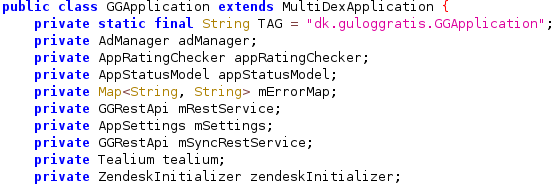
\includegraphics[width=1\columnwidth]{../static-analysis/pictures/GGApplication_properties.png}
    \caption{Part of GGApplication class}
    \label{fig:ggapplication-properties}
\end{figure}

This is a snippet from the start of a class, that initializes services and makes them available across the application. There is neither use of name obfuscation nor string encryption. As a consequence it is easy for an adversary to understand the code flow and in this case identify some of the services used in the application.

To ease the static analysis \href{https://github.com/MobSF/Mobile-Security-Framework-MobSF}{MobSF}\footnote{\href{https://github.com/MobSF/Mobile-Security-Framework-MobSF}{https://github.com/MobSF/Mobile-Security-Framework-MobSF}} is used to identify known flaws and vulnerabilities. MobSF gives the application a security score of 35/100, which might indicate that there is some vulnerabilities. Looking at the report there are several configurations, that is tagged as medium or high severity. One is the allowance of application data backup. This is a flag that defaults to true. If sensitive data is stored this should be considered actively set to false. The code analysis shows an extensive amount of logging. Examples of this can been seen in a search on Figure \ref{fig:log-payments}.

\begin{figure}[htbp]
    \centering
    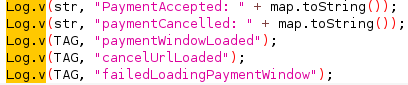
\includegraphics[width=1\columnwidth]{../static-analysis/pictures/log_payments.png}
    \caption{Search of log statements}
    \label{fig:log-payments}
\end{figure}

These log statements are called in callback functions from an external library containing Dibs logic. Dibs is basically NETS which is used to perform payments. These log statements can contain sensitive payment information and should not be included in a release build. A way to avoid this is using \href{https://github.com/JakeWharton/timber}{timber}\footnote{\href{https://github.com/JakeWharton/timber}{https://github.com/JakeWharton/timber}}. Timber is a wrapper that enables the possibility of only enabling log statements in debug builds. Timber is used for some parts of the application but neglected in other parts.    

Another potential flaw is seen in the Dibs library. The library utilizes a webViewClient, which is embedding a browser in the application. The code can be seen on Figure \ref{fig:dibs-webview}. The code enables Javascript in the embedded browser and adds an interface to Java code. This is a known vulnerability to all Android sdk versions below 17\cite{avg-webview-explot}. This is not an issue, since the application has a minimum sdk version of 21.    

\begin{figure}[htbp]
    \centering
    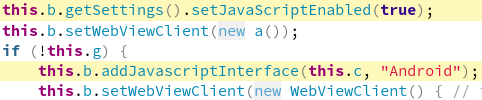
\includegraphics[width=1\columnwidth]{../static-analysis/pictures/dibs-javascript.png}
    \caption{Dibs library embedded webview}
    \label{fig:dibs-webview}
\end{figure}

Another webview vulnerability is seen the Zendesk library. This can be seen on Figure \ref{fig:zendesk-webview}. Here the webview allows debugging. This means it is possible to attach an debugger and see/control the execution of the webview.    

\begin{figure}[htbp]
    \centering
    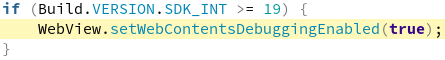
\includegraphics[width=1\columnwidth]{../static-analysis/pictures/zendesk-webview.png}
    \caption{Zendesk library embedded webview}
    \label{fig:zendesk-webview}
\end{figure}

The report from MobSF as well display the use of SSL pinning. This can be seen on Figure \ref{fig:ssl-pinning} and will be analysed later in the attempt of a man-in-the-middle attack. 

\begin{figure}[htbp]
    \centering
    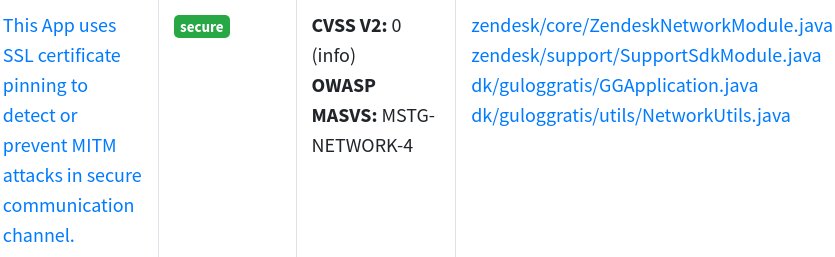
\includegraphics[width=1\columnwidth]{../static-analysis/pictures/ssl-pinning.png}
    \caption{Usage of SSL pinning}
    \label{fig:ssl-pinning}
\end{figure}

\subsection{Dynamic Analysis}
A dynamic analysis was performed using MobSF. An emulator with sdk version 29 is spawned locally using \href{https://www.genymotion.com/}{genymotion}\footnote{\href{https://www.genymotion.com/}{https://www.genymotion.com/}}. MobSF then installs an instrumented version with configurations of our choice. The defaults are selected which includes: installing root certificate, setup HTTPs proxy, SSL pinning bypass, etc. Then some execution flows are performed on the device and a report is generated. It is then possible to see various information of the execution. The network traffic can be seen. These requests are sent to \href{https://portswigger.net/burp}{Burp Suite}\footnote{\href{https://portswigger.net/burp}{https://portswigger.net/burp}}, and will be analysed in the next section. The host names and their geolocation can be seen together with trackers. It is also possible to see log statements. A example can be seen on Figure \ref{fig:log-login-request}. It shows that URLs together with query parameters are logged.  

\begin{figure}[htbp]
    \centering
    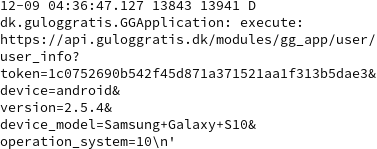
\includegraphics[width=1\columnwidth]{../static-analysis/pictures/log-login-request.png}
    \caption{Logging HTTP request}
    \label{fig:log-login-request}
\end{figure}

The generated report also shows the local files stored in the applications own data directory. An example is a XML file stored in SharedPreferences. A snippet of the file can be seen on Figure \ref{fig:gull-prefs-xml}. It is seen that the token stored is the one used in HTTP requests.  

\begin{figure}[htbp]
    \centering
    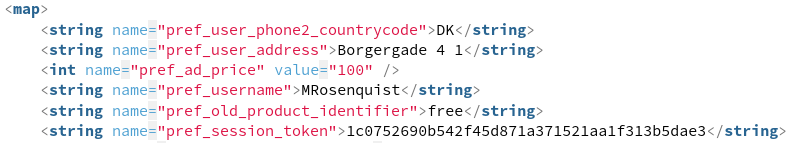
\includegraphics[width=1\columnwidth]{../static-analysis/pictures/gull-prefs-xml.png}
    \caption{Part of xml preference file}
    \label{fig:gull-prefs-xml}
\end{figure}

\section{Network Security}
In the dynamic analysis the host names were reported. The application has many external dependencies, but the domain we are primarily interested in is, \textit{api.guloggratis.dk}. This is the api responsible of the business logic and data. The server's TLS configuration is analysed with \href{https://www.ssllabs.com}{Qualys SSL Labs}\footnote{\href{https://www.ssllabs.com}{https://www.ssllabs.com}}. The overview can be seen on figure \ref{fig:sslreport-overview}. It is seen the server supports old version of TLS, weak ciphers and handshakes. The certificate is issued by Cloudflare and it is only domain validated. Meaning it only proves they are the owner of the site but there is no organization information required to achieve such a certificate.  

\begin{figure}[htbp]
    \centering
    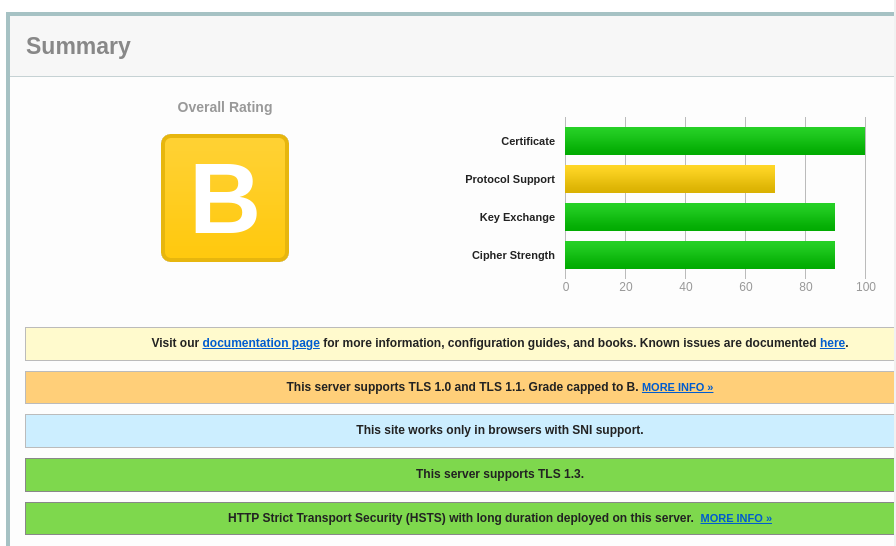
\includegraphics[width=1\columnwidth]{../static-analysis/pictures/sslreport_overview.png}
    \caption{TLS configuration of server}
    \label{fig:sslreport-overview}
\end{figure}

An attempt of performing a man-in-the-middle attack will be conducted. This revolves around setting us between the application and the server which it is communicating with. This was already performed in the dynamic analysis using MobSF. Instead of using MobSF we will do the instrumentation and configuration ourselves to fully understand the behaviour. The setup consists with the same emulator as before but now with Burp Suite as the proxy. Firstly, we install the apk, disable data and proxy the Wi-Fi to Burp Suite. Then the app is started and resulting in the TLS handshake failing. This is because the phone does not trust Burp Suite's certificate. The certificate is then installed in the emulators trust store. Then traffic can be intercepted in the emulators browser but the TLS connection still fails in the application. This is caused by either SSL pinning or certificate transparency. Remembering from the static analysis MobSF showed that this was present. Delving into the decompiled code it is seen that certificate transparency is used for the main server. The code can be seen on figure \ref{fig:retrofit-ct}

\begin{figure}[htbp]
    \centering
    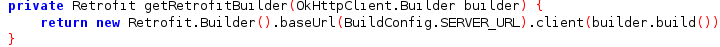
\includegraphics[width=1\columnwidth]{../static-analysis/pictures/retrofit-okkhtp-builder.png}
    \caption{Retrofit builder implementing certificate transparency with OkHttp}
    \label{fig:retrofit-ct}
\end{figure}

It is not apparent that certificate transparency is implemented here. However building Retrofit on top of OkHttp activates certificate transparency\cite{android-certificate-transparency}. Thus some bypassing is necessary. It is unclear how MobSF performed this bypass, but it uses \href{https://frida.re/docs/android/}{Frida}\footnote{\href{https://frida.re/docs/android/}{https://frida.re/docs/android/}}, which has several tools for this purpose. We will instead try with a patched apk generated with \href{https://github.com/shroudedcode/apk-mitm}{apk-mitm}\footnote{\href{https://github.com/shroudedcode/apk-mitm}{https://github.com/shroudedcode/apk-mitm}}. Success, it is now possible to intercept traffic in Burp Suite. The generated request from the dynamic analysis is then sent to Burp Suite for extra foundation. Multiple execution flows are performed. The traffic is then investigated. An overview of some requests can be seen on figure \ref{fig:http-requests-modules}    

\begin{figure}[h!]
    \centering
    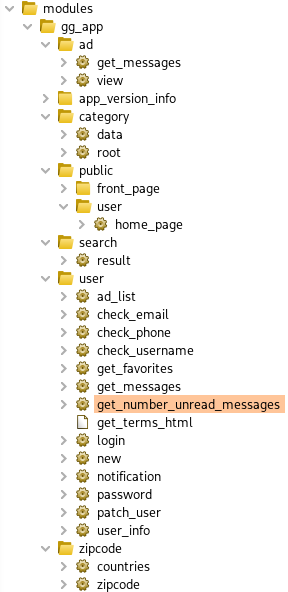
\includegraphics[width=0.5\columnwidth]{../dynamic-analysis/pictures/http-requests-modules.png}
    \caption{HTTP Requests for $<$host name$>$/modules/}
    \label{fig:http-requests-modules}
\end{figure}

Having the setup running it is now possible to perform an attack. Looking at the example of setting an item for sale. We know by analysing the code and requests we want to intercept \textit{modules/gg\_app/ad/} requests. The interception can be seen on figure \ref{fig:attack-new-ad}. The headline and description is than changed to \textit{mitm}. The resulting item can be seen on figure \ref{fig:attack-final-ad}.  

\begin{figure}[htbp]
    \centering
    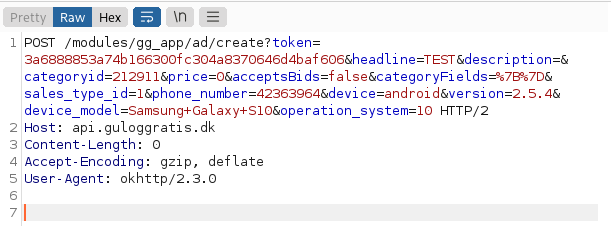
\includegraphics[width=1\columnwidth]{../dynamic-analysis/pictures/MITM-auction-burp.png}
    \caption{Create new ad request}
    \label{fig:attack-new-ad}
\end{figure}

\begin{figure}[htbp]
    \centering
    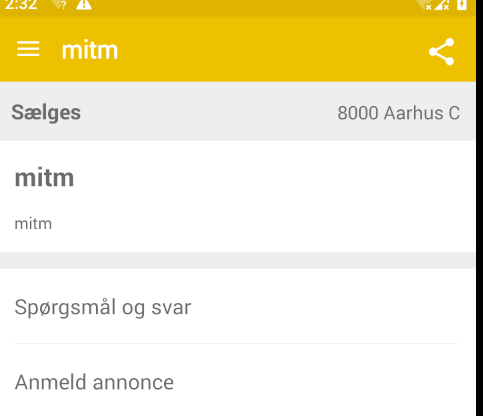
\includegraphics[width=0.5\columnwidth]{../dynamic-analysis/pictures/mitm_auction.png}
    \caption{Manipulated final item}
    \label{fig:attack-final-ad}
\end{figure}

This is an example of manipulating the requests moving from client to server. Burp Suite allow us to also manipulate the response. A result of this can be seen on figure \ref{fig:server-client-mitm}. Here the JSON received from server is manipulated.  

\begin{figure}[htbp]
    \centering
    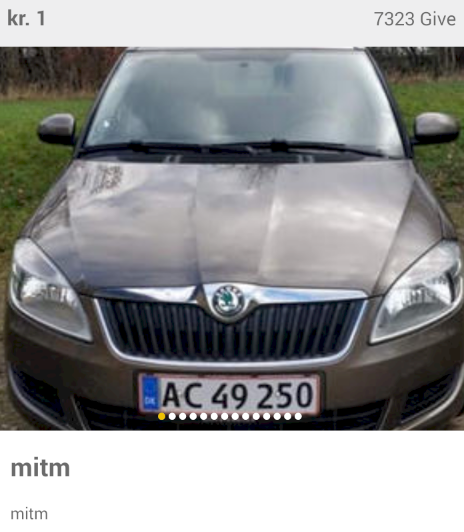
\includegraphics[width=0.5\columnwidth]{../dynamic-analysis/pictures/server-client-mitm.png}
    \caption{Manipulated response from server}
    \label{fig:server-client-mitm}
\end{figure}

In general the networking between application and server is quite easy to understand. It is not a standard REST api which follows all the standards. It is routed by \textit{modules/gg\_app/$<$entity$>$/$<$action$>$}. An example can be seen for the \textit{ad} entity on figure \ref{fig:ad-actions}. 

\begin{figure}[htbp]
    \centering
    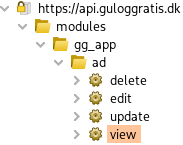
\includegraphics[width=0.5\columnwidth]{../dynamic-analysis/pictures/ad-actions.png}
    \caption{Example of actions for the ad entity}
    \label{fig:ad-actions}
\end{figure}

The HTTP methods are not used as expected. An example is that deleting an ad is done with a GET request. In general the nature of the traffic is the application targeting an action with some query parameters and then the server returning some JSON.    

\section{Authentication}
It is essential for the users of the application to have accounts. It enables user interaction and many of the features that are desired in a marketplace application. User's expect their actions and settings persisted across platforms. However, they expect some privacy. Other users should not be able to see their private details. This all leads to the need of having authentication methods in the application. The way it is handled in the application is by allowing three authentication methods: Facebook, Google and email address. Going forward we will only look at email address, as that is GulOgGratis own implementation. 

When you create an account the default information is entered and you press create. Looking at the network traffic some validation of various fields are performed. An example is verifying the email is not in use. The application then sends the information to the server, an account is created, the application performs a login request and the server returns tokens. However the email was never verified. The server returns a JWT (JSON Web Token) and another token consisting of forty characters. A decoded JWT can be seen on figure \ref{fig:jwt_decoded}. The header indicates that the token is signed using HMAC-SHA256 and the payload contains some user information. It is unclear looking at the network traffic and the source code what the JWT is used for. Meanwhile the other undefined token is stored locally and used in every HTTP request.  

\begin{figure}[htbp]
    \centering
    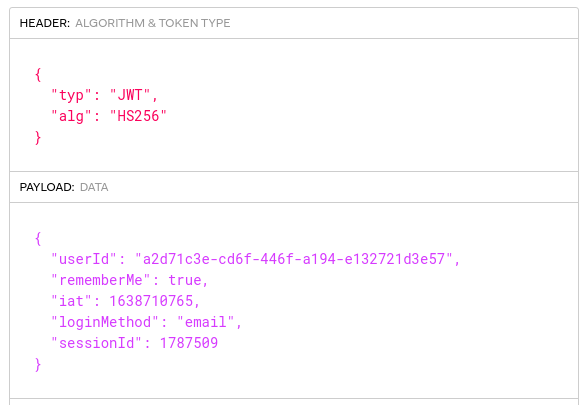
\includegraphics[width=0.7\columnwidth]{../dynamic-analysis/pictures/jwt_decoded.png}
    \caption{Decoded JSON Web Token}
    \label{fig:jwt_decoded}
\end{figure}

Having created the account you can sign in using your email and password. The application then calls the api with a login action and the tokens are returned. The user is then authenticated and ready to use them for further actions. The used token is persisted in the application's local directory. When the user then signs out no network traffic is detected. However looking at the code it is seen that the token, user address and user id are removed from local storage.      

The password used for authenticating is quite unrestricted. The only requirements are that they need to be at least eight signs and a combination of numbers and letters. Additionally, when changing the password it is allowed to change to one that has already been used, and changing it to the exact same. Resetting the password results in no received email even though a request is detected. Trying to perform the reset on the web site results in an instantaneous received email. Inspecting that traffic it is interesting to see that it utilizes another hostname and the request is completely different. This might indicate that the API the mobile application utilizes is becoming obsolete.     

In the system it is possible to validate your account with NemID. This ensures you are the person who you indicate you are. This is a safety for others interacting with you. The validation can only happen through the web site. 



\section{Privacy}
Mobile applications have the potential of collecting massive amount of data from their users. This can be used to increase user experience but also lead to intrusive behaviour. Permissions is a great place to see if something is out of the ordinary. Some of the most interesting permissions related to privacy of the application:  

\begin{itemize}
    \item INTERNET \& ACCESS NETWORK STATE
    \item MANAGE ACCOUNTS \& GET ACCOUNTS \& USE CREDENTIALS
    \item ACCESS FINE LOCATION \& ACCESS COARSE LOCATION
\end{itemize}

The networking permissions are obviously necessary. The account permissions are used to authenticate with either Google or Facebook. The most interesting are the location related. When opening the application the user is prompted whether he will allow location tracking when using the app. This setting is persistent and can not be disabled from the application. The user has to disable it in settings. Additionally, there should be an option to allow for one session. The location permission does not seem necessary for the application. The only use is related to a map shown on items for sale. As Google Maps is used for this feature it might be a needed permission.

The data collection of the application revolves around how users use the application and advertisement. Almost whenever button is pressed a chain of requests are performed. A chain can be seen on Figure \ref{fig:statistics-chain}. 

\begin{figure}[htbp]
    \centering
    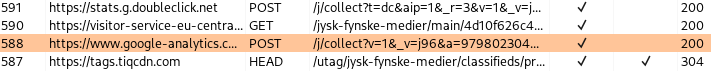
\includegraphics[width=1\columnwidth]{../static-analysis/pictures/statistics_trackview_chain.png}
    \caption{Analytics chain on user actions}
    \label{fig:statistics-chain}
\end{figure}

An example of the request can be seen on Figure \ref{fig:statistic-request-car}. This request is triggered by the car category when searching for items.  

\begin{figure}[htbp]
    \centering
    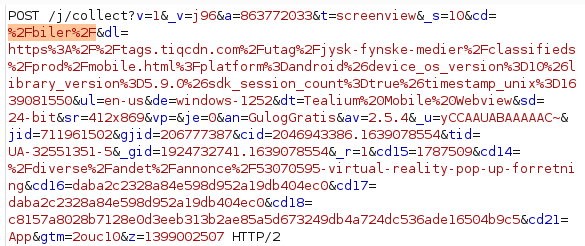
\includegraphics[width=1\columnwidth]{../dynamic-analysis/pictures/analytics-request-cars.png}
    \caption{Analytics request when pressed on the cars(biler) category}
    \label{fig:statistic-request-car}
\end{figure}

These requests send the user's actions to external services. It is seen that the event is sent to Google Analytics and Doubleclick. Doubleclick is an advertisement company owned by Google. This result in targeted advertisements for the user dependent on his behaviour in the application. There is a range of trackers. An overview can be seen on Table \ref{tab:trackers}. 

\begin{table}[]
    \centering
    \begin{tabular}{|l|l|l|}
    \hline
    \textbf{Company} & \textbf{Tracker Name} & \textbf{Category} \\ \hline
    Facebook         &                       &                   \\ \hline
                     & Ads                   & Advertisement     \\
                     & Analytics             & Analytics         \\
                     & Audience              & Analytics         \\ \hline
    Google           &                       &                   \\ \hline
                     & AdMob                 & Advertisement     \\
                     & Analytics             & Analytics         \\
                     & CrashLytics           & Crash reporting   \\
                     & DoubleClick           & Advertisement     \\ \hline
    Tealium          &                       & Analytics         \\ \hline
    \end{tabular}
    \caption{Overview of some of the trackers}
    \label{tab:trackers}
\end{table}

The analytics trackers are used to improve user experience. Looking at metrics regarding user sessions and actions. CrashLytics is used to report crashes and tell the developers the state of the application at the incident. The advertisement trackers are retrieving information from the users behaviour and thus targeting advertisements thereof. If the user authenticates with both Facebook and Google, it is expected that the tracking goes beyond the scope of this application. Meaning the behaviour of the user might be visual in ads he receives on other platforms. Other than that there is no integration to social networks.       

\section{Discussion}
Retrieving a basic understanding the code and flow of the application did not require much time. This is the result of not utilizing obfuscation when compiling the release build. As per the documentation\cite{android-obfuscation} this does not require a lot of effort. It is done by enabling Proguard in the build.gradle. Extensive logging is as well present. This might be of no harm but for a release build these should not be present. Lack of obfuscation and logging only gives an adversary an unnecessary edge in finding potential vulnerabilities. External libraries might be the attack vector for an attacker. He might know a vulnerable library and target a application using it. The Dibs and Zendesk library both utilized a embedded view. One added an interface to call Java code from javascript while the other allowed debugging. The interface has been known to be dangerous. If an adversary where to control the Javascript called from the webview, he would be able to perform severe attacks. However, this was patched in sdk version 17 and the minimum sdk version is 21 for the application.

The TLS configuration of the server resulted in a decent rating. Though, the support for TLS 1.0 and TLS 1.1 should be deactivated. The targeted api versions of the application all support TLS 1.2\cite{android-sslsocket}. The certificate of the server is only domain validated. This is the lowest amount of validation. Users know their data is encrypted however they cant truly trust who is at the receiving end. The certificate should be at least be upgraded to organization validated.

In the attempt of the man-in-the-middle attack there was hurdles. The device has to trust the proxy's certificate and a patched apk is required. This might not be realistic to pull of on an user's device. However, an adversary can mount severe attacks if he is to achieve the setup. The attacks he can perform is editing requests/response, DOS or just eavesdropping. All these are extremely critical and combined violates all policies. In understanding the network traffic an adversary did not need to mount a man-in-the-middle attack, he could just use the application himself.

A token stored in the application local directory are used for each request. Backups of the application data is allowed. Meaning if an adversary are to retrieve a backup of the data, he would be able to perform requests on the user's behalf. This could potentially be avoided by encrypting the token. The token is retrieved by authenticating in the application. First time users creates their account. Leading to immediate authentication with no email confirmation. This is flaw and results in users being able to create accounts with other persons' emails. Additionally, the passwords are allowed to be quite weak and it is possible to change your password to the same or reusing older ones. This encourages brute force attacks. After having authenticated in the application the token is stored and used in further sessions. Therefore, if the phone is unlocked anyone can access the application. This could be resolved by introducing "something you are" authenticity in the form of finger or face scan. Currently the application only uses "something you know" and keeps the user authenticated after first sign in.  

The application is not as intrusive as witnessed from other horror stories. The permissions is quite ordinary and expected. However, location permission handling could be improved. There should be transparency in what the permission is used for and it should be possible to limit it for sessions. Advertisements are shown in the application and they are personalized by a range of trackers. These trackers retrieve continuous data from the users' behaviour. This is sort of expected from nowadays applications. But it should be described in a Privacy Policy or Terms and Condition accessible for the user. These are nowhere to be found in the application.

\section{Conclusion}
A preliminary security analysis was performed on GulOgGratis' Android application. The analysis was conducted on the basis of a constructed threat model. It was broken down to four different aspects and it was shown that there are flaws more severe then others. Simple mechanisms should be implemented to harden adversaries achieving insight in their application. Improvements can be made in regards of network traffic, authentication methods and privacy transparency. The application is not vulnerable to any apparent and simple to pull of exploits. However, an adversary with a strong motivation might be able to mount an attack. Either by performing a man-in-the-middle attack or stealing the user's token. This would result in a complete violation of almost all security properties.      

\printbibliography
\end{document}